\newpage
\section{Definition of Mass Transfer}

\subsection*{Resources}
\begin{itemize}
    \item Chapter 14, introduction
\end{itemize}

\subsection*{Challenge}
Add the points of the following conditions which constitute diffusive mass-transfer

1 point: Evaporation of water vapour into the air

2 points: Water being pumped through a pipe

4 points: Dissolving of sugar into tea

8 points: Aeration of waste-water

16 points: Motion of air around a room due to the presence of a fan

\subsection*{Solution}
\solint{a}{d16142}




\newpage
\section{Diffusion in the long time limit}

\subsection*{Resources}
\begin{itemize}
    \item Book: 14.1.1 to 14.1.2
    \item Video: \url{https://www.youtube.com/watch?v=-FLv0uxLrDI}
\end{itemize}

\subsection*{Challenge}
Consider a box of volume \SI{1}{\cubic\meter}. The box contains 1 mole of gas. At time $t=0$, all the gas molecules in the left 1/4 of the box are labeled $A$. As time goes to $t=\infty$, what will the density of the molecules labeled $A$ be in the right half of the box? Note that there is only 1 species of gas in the box.

\subsection*{Solution}
(Units: Moles / $m^3$)

\soltwodp{b}{e1f90a}




\newpage
\section{Definitions of quantities I}

\subsection*{Resources}
\begin{itemize}
    \item Book: 14.1.1 to 14.1.2
    \item Video: \url{https://www.youtube.com/watch?v=-FLv0uxLrDI}
\end{itemize}

\subsection*{Challenge}
Assuming air is made up exclusively of oxygen and nitrogen with their partial pressures in the ratio 0.21:0.79, what are their mass-fractions?

\subsection*{Solutions}
Oxygen: 0.233 \\
Nitrogen: 0.767




\newpage
\section{Definitions of quantities II}

\subsection*{Resources}
\begin{itemize}
    \item Book: 14.1.1 to 14.1.2
    \item Video: \url{https://www.youtube.com/watch?v=-FLv0uxLrDI}
\end{itemize}

\subsection*{Challenge}
Japan imports substantial amounts of LNG which is a mixture of the following gases:

\begin{tabular}[c]{|c|c|}
    \hline
    \textbf{Liquid} & \textbf{Mol \%}\\
    \hline
    Methane         & 93.5  \\
    Ethane          & 4.6   \\
    Propane         & 1.2   \\
    Carbon dioxide  & 0.7   \\
    \hline
\end{tabular}

The masses of Methane, Ethane, Propane and Carbon Dioxide are 16, 30, 44 and 44 g/mol respectively.

Assuming ideal gases, calculate the following:

1. The mole-fraction of ethane

2. The mass-fraction of ethane

3. The average molecular mass of the mixture

4. The mass-density of the gas when heated to \SI{207}{\kelvin} under a total pressure of \SI{1.4e5}{\pascal}

5. The partial pressure of the methane when the total pressure is \SI{1.4e5}{\pascal}

\subsection*{Solutions}

\textbf{1.}\\
\solthreedp{c}{bf4ce8}

\textbf{2.}\\
\solthreedp{d}{d34e49}

\textbf{3.} (Units: g/mol)\\
\soltwodp{e}{6b58f1}

\textbf{4.}\\
\SI{1397}{\gram\per\cubic\meter}

\textbf{5.} (Units: kPa)\\
\solint{f}{4d1d94}




\newpage
\section{Mass diffusivity}

\subsection*{Resources}
\begin{itemize}
    \item Book: 14.1.3 - 14.1.4, Table A-8
\end{itemize}

\subsection*{Challenge}
Estimate the mass diffusivity of the following gases in air at 350 K and 1 atm pressure:

1. Ammonia\\
2. Hydrogen

\subsection*{Solutions}
1. \SI{3.6e-5}{\square\meter\per\second}\\
2. \SI{5.2e-5}{\square\meter\per\second}




\newpage
\section{Cases of diffusion}

\subsection*{Resources}
\begin{itemize}
    \item Book: 14.1.3 - 14.1.4
\end{itemize}

\subsection*{Challenge}
Considering air as a mixture of two gases ($O_2$ and $N_2$), situated in a closed, cylindrical container with its axis vertical and with opposite ends maintained at different temperatures. Assume the total pressure of the air is uniform throughout the container.

Consider each of the following conditions:

A) The bottom surface is colder than the top surface\\
B) The top surface is colder than the bottom surface

\vspace{1cm}
1. Add the points for the following \emph{true} statements:

\textbf{1 point} There is motion of the air in case (A)

\textbf{2 points} There is no motion of the air in case (A)

\textbf{4 points} There is motion of the air in case (B)

\textbf{8 points} There is no motion of the air in case (B)

\textbf{16 points} There is diffusive mass transfer inside the cylinder in case (A)

\textbf{32 points} There is no diffusive mass transfer inside the cylinder in case (A)

\textbf{64 points} There is diffusive mass transfer inside the cylinder in case (B)

\textbf{128 points} There is no diffusive mass transfer inside the cylinder in case (B)

\vspace{1cm}
2. Explain your reasoning

\subsection*{Solutions}
\textbf{1.}\\
\solint{g}{389975}

\textbf{2.}\\
Please compare your answer with your partner in class.




\newpage
\section{Diffusion coefficient equivalency}

\subsection*{Resources}
\begin{itemize}
    \item Video: \url{https://www.youtube.com/watch?v=NTlR18NyqAE}
\end{itemize}

\subsection*{Challenge}
Prove that in a binary mixture, the diffusion coefficient of gas ``A'' in ``B'' is the same as the diffusion coefficient of gas ``B'' in ``A'' (ie, $D_{AB} = D_{BA}$).




\newpage
\section{Column evaporation derivation}

\subsection*{Resources}
\begin{itemize}
    \item Book 14.2
\end{itemize}

\subsection*{Challenge}
Starting from basic knowledge of absolute flux in terms of both diffusion and advection:
\begin{equation}
    N''_A = -C D_{AB} \Delta x_A + x_A N''_A
\end{equation}
show that evaporation in a stationary column (figure 14.2 in the book) can be given by
\begin{equation}
    N''_A = \frac{C D_{AB}}{L} ln \left( \frac{1-x_{A,L}}{1-x_{A,0}} \right)
\end{equation}
where $x_{A,L}$ and $x_{A,0}$ are the molar fractions at the top and bottom the column, respectively.


\subsection*{Solution}
Compare your answer with your partner




\newpage
\section{Saturated water vapour pressure}

\subsection*{Resources}
\begin{itemize}
    \item \url{http://www.chemguide.co.uk/physical/phaseeqia/vapourpress.html}
    \item \url{https://sciencing.com/water-vapor-pressure-vs-humidity-19402.html}
\end{itemize}

\subsection*{Challenge}
\textbf{1)} Write a few sentences briefly explaining what is meant by ``Saturated Vapour Pressure'' and how it is related to ``Relative humidity''.

\textbf{2)} Considering an air-water interface at equilibration, if the relative humidity is 50\% and the saturated water density is \SI{0.02}{\kmol\per\cubic\meter}, what is the density of water vapour near the interface? In addition to a numerical answer, explain in a few words the reasoning behind your answer.

\textbf{3)} Under the same conditions as part (2), what is the mole-fraction of water vapour above the surface? You may assume a temperature of \SI{2}{\celsius} and an atmospheric pressure of $1$ atmosphere.

\textbf{4)} Considering the saturation pressure of water is 0.03 atm, what is the mole-fraction of water vapour in the air at 1 atm when the humidity is 100\%? (You may assume an ideal gas.)

\subsection*{Solution}
\textbf{1)}\\
Compare your answer with your partner.

\textbf{2)}\\
(Units: \si{\kmol\per\cubic\meter})\\
\soltwodp{a}{9bb791}

Compare your reasoning with your partner.

\textbf{3)}\\
\soltwodp{b}{06ac46}

\textbf{4)}\\
\soltwodp{c}{f2a860}




\newpage
\section{Evaporation through a pore}

\subsection*{Resources}
\begin{itemize}
    \item Book 14.2
\end{itemize}

\subsection*{Challenge}
In your challenge log, work through example 14.2 (you do not need to include the ``comments'' part in your challenge log).




\newpage
\section{Evaporation pan}

\subsection*{Resources}
\begin{itemize}
    \item Book 14.2, Table A-8
\end{itemize}

\subsection*{Challenge}
Evaporation pans like the one shown are used to measure the rate of evaporation of water in a local area.

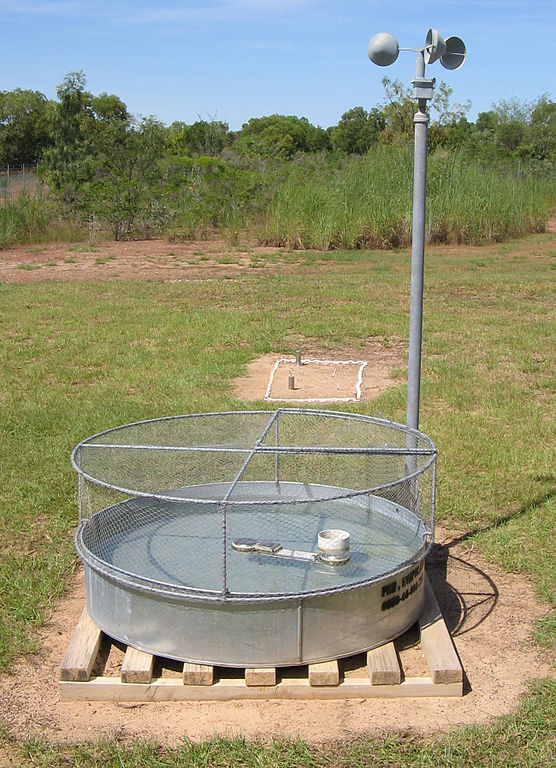
\includegraphics[height=8cm]{evappan}
\emph{(image: \href{https://commons.wikimedia.org/wiki/File:Evaporation_Pan.jpg}{Bidgee, Wikipedia)}}

An evaporation pan is placed in a location with an ambient air temperature of \SI{298}{\kelvin} and relative humidity of 25\%. The pan contains water at the same temperature as the surrounding air. The pan has a diameter of \SI{20}{\cm} and height of \SI{160}{\mm}, and it starts half-full of water.

1. Assuming only diffusive mass transport, what is the initial evaporation rate?

2. Including the effects of advection, what is the initial evaporation rate?

(The saturation pressure of water at \SI{298}{\kelvin} is \SI{0.03531}{\bar}, and its specific volume at an atmospheric pressure of  1 atm is \SI{39.13}{\meter\cubed\per\kilogram}.)

\subsection*{Solution}
1. \SI{1.087e-8}{\kilo\mol\per\second}\\
2. \SI{1.116e-8}{\kilo\mol\per\second}





\newpage
\section{Stationary Medium}

\subsection*{Resources}
\begin{itemize}
    \item Video: \url{https://www.youtube.com/watch?v=F0deXOH_YEM}
\end{itemize}

\subsection*{Challenge}
\begin{enumerate}
    \item Briefly explain what is meant by a stationary medium.
    \item Considering a stationary medium of 3 species ``A'', ``B'' and ``C'' with equal molar concentration, if the flux of species ``A'' is \SI{2}{\kmol\per\square\meter\per\second} and ``B'' is \SI{-8}{\kmol\per\square\meter\per\second}, what is the flux of species ``C''?
    \item Considering a binary system of atoms ``A'' and ``B'' with concentration \SI{5}{\kmol\per\cubic\meter} and \SI{10}{\kmol\per\cubic\meter} respectively, if the molar velocity of species ``A'' is \SI{2}{\meter\per\second}, what is the molar velocity of species ``B''?
\end{enumerate}



\subsection*{Solutions}
\textbf{1.}\\
Please compare your answer with your partner.

\textbf{2.}\\
(Units: \si{\kmol\per\square\meter})\\
\solint{g}{4a4314}

\textbf{3.}\\
(Units: \si{\meter\per\second})\\
\soltwodp{h}{5ba818}




\newpage
\section{Stationary Medium Approximation}

\subsection*{Resources}
\begin{itemize}
    \item Book 14.3
\end{itemize}

\subsection*{Challenge}
In a few sentences, describe what is meant by \emph{the stationary medium approximation}. Give at least one real-world example each of case where the stationary medium approximation would and would-not be appropriate.

\subsection*{Solution}
Compare your answer with your partner




\newpage
\section{Steady-state definition}

\subsection*{Resources}
\begin{itemize}
    \item Web: \url{http://www.virginia.edu/bohr/mse209/chapter5.htm}
\end{itemize}

\subsection*{Challenge}
1. Write a sentence or two explaining what is meant by steady-state conditions in this context.

2. What is $\delta J(x) / \delta t$ at any given position $x$ under a steady-state condition?

\subsection*{Solutions}
\textbf{1.}\\
Please compare your answer with your partner

\textbf{2.}\\
\soltwodp{a}{690969}




\newpage
\section{Steady-state diffusion planer example I}

\subsection*{Resources}
\begin{itemize}
    \item Book: 14.4.1 to 14.4.3
    \item Video: \url{https://youtu.be/4KACai1gYzc}
\end{itemize}

\subsection*{Challenge}
Work through the calculation from equations 14.51 to 14.54, showing your reasoning along the way. Don't worry about the concept of diffusion resistance for now.




\newpage
\section{Steady-state diffusion planer example II}

\subsection*{Resources}
\begin{itemize}
    \item Book: 14.4.1 to 14.4.3
    \item Video: \url{https://youtu.be/4KACai1gYzc}
\end{itemize}

\subsection*{Challenge}
Work through example 14.3 in section 14.4.3.




\newpage
\section{Steady-state diffusion through flat surface}

\subsection*{Resources}
\begin{itemize}
    \item Book: 14.4.1 to 14.4.3
\end{itemize}

\subsection*{Challenge}
A thin plastic membrane is used to maintain separation between helium and an outer chamber. Under steady-state conditions, the concentration of helium is \SI{0.02}{\kmol\per\cubic\meter} and \SI{0.005}{\kmol\per\cubic\meter} at the inner and outer boundaries respectively. If the membrane is \SI{1}{\mm} thick and the binary diffusion coefficient of helium in the plastic membrane is \SI{e-9}{\square\meter\per\second}, what is the diffusive flux through the membrane in terms of \si{\kmol\per\second\per\square\meter} and \si{\kg\per\second\per\square\meter}?

\subsection*{Solution}
\SI{1.5e-8}{\kmol\per\second\per\square\meter}\\
\SI{6.0e-8}{\kg\per\second\per\square\meter}




\newpage
\section{Steady-state diffusion in pipe walls}

\subsection*{Resources}
\begin{itemize}
    \item Book: 14.4.1 to 14.4.3
\end{itemize}

\subsection*{Challenge}
A pipe with inner-radius \SI{10}{\cm} and outer-radius \SI{13}{\cm} is carrying hydrogen. The concentration of hydrogen inside the pipe is \SI{0.07}{\kmol\per\cubic\meter} and outside the pipe is \SI{0.04}{\kmol\per\cubic\meter}. If the hydrogen has a diffusion coefficient of \SI{e-8}{\square\meter\per\second} in the walls of the pipe, at what rate is hydrogen lost from the pipe, per metre length of pipe?

\subsection*{Solution}
\SI{7.18e-9}{\kmol\per\second}




\newpage
\section{Raoult's law}

\subsection*{Resources}
\begin{itemize}
    \item Book: 14.5.1
\end{itemize}

\subsection*{Challenge}
Given that the saturated vapour pressure of water in the atmosphere at \SI{17}{\celsius} is \SI{0.01917}{\bar}, considering a puddle of water exposed to the atmosphere at \SI{17}{\celsius}, calculate the following. You may assume that the average mass of air is \SI{29}{\gram\per\mol}.

1. The molar fraction of water vapour on the air-side of the water-air interface.\\
2. The mass fraction of water vapour on the air-side of the water-air interface.\\
3. The molar fraction of water vapour on the water-side of the water-air interface.\\
4. The mass fraction of water vapour on the water-side of the water-air interface.

\subsection*{Solution}
1. \num{0.019}

2. \num{0.012}

3.\\
X = Your solution\\
Form: Decimal, to 3 decimal places\\
Place the indicated letter in front of the number\\
Example: aX where $X=42.544$ is entered as \href{http://www.wolframalpha.com/input/?i=md5+hash+of+\%22a42.544\%22}{a42.544}

hash of bX = 4b5ab9

4.\\
X = Your solution\\
Form: Decimal, to 3 decimal places\\
Place the indicated letter in front of the number\\
Example: aX where $X=42.544$ is entered as \href{http://www.wolframalpha.com/input/?i=md5+hash+of+\%22a42.544\%22}{a42.544}

hash of cX = d69d92




\newpage
\section{Boundary conditions}

\subsection*{Resources}
\begin{itemize}
    \item Book: First page of section 14.5
\end{itemize}

\subsection*{Challenge}
State two different types of boundary conditions in terms of molar density, $x_i$.

\subsection*{Solution}
Please discuss with your partner and the teacher.




\newpage
\section{Henry's law}

\subsection*{Resources}
\begin{itemize}
    \item Book: 14.5.2
\end{itemize}

\subsection*{Challenge}
Consider a gas stream flowing above a liquid. Species $A$ has a mole fraction of \num{0.5} in the liquid while species $B$ has a mole fraction of \num{0.005} in the liquid. Calculate Henry's constant for the gas where Henry's law is most applicable, if the partial pressure of both species in the gas stream is \SI{0.5}{\bar}.

\subsection*{Solution}
\hashnew{1}{}{5}{f}{4e930b} % Decimal places, ``s'' in places, 42.X, hash letter, hash




\newpage
\section{Solubility}

\subsection*{Resources}
\begin{itemize}
    \item Book: 14.5.2
\end{itemize}

\subsection*{Challenge}
1. Considering a solid-gas interface, calculate the solubility of species \emph{A} if the density of \emph{A} is \SI{e-3}{\kmol\per\cubic\meter} in the solid given a partial pressure of \SI{0.5}{\bar} in the gas.

2. What volume will species \emph{A} occupy in the gas-phase at STP if it occupies \SI{20}{\cubic\meter} in the solid phase?

\subsection*{Solution}
1.\\
X = Your solution\\
Units: kmol / $m^3$ (solid) / bar (partial pressure in gas phase)\\
Form: Scientific notation with the mantissa in standard form to 1 decimal place and the exponent in integer form\\
Place the indicated letter in front of the number\\
Example: aX where $X=4.0 \times 10^{-3}$ is entered as \href{http://www.wolframalpha.com/input/?i=md5+hash+of+\%22a4.0e-3\%22}{a4.0e-3}

hash of gX = 0174a0

2. \SI{0.908}{\cubic\meter}




\newpage
\section{Flux through membrane with solubility}

\subsection*{Resources}
\begin{itemize}
    \item Book: 14.5.2
\end{itemize}

\subsection*{Challenge}
Work through example 14.4




\newpage
\section{Flux through spherical membrane}

\subsection*{Resources}
\begin{itemize}
    \item Book: 14.5.2
\end{itemize}

\subsection*{Challenge}
Consider helium gas stored in a silicon spherical container at \SI{25}{\celsius} and \SI{4}{\bar} pressure, with an inner radius of \SI{100}{\mm} and outer radius of \SI{110}{\mm}. Calculate the rate at which it escapes from the container. Assume a diffusion coefficient of helium in the walls of the container of \SI{0.4e-13}{\square\meter\per\second} and a solubility of Helium in Silicon of \SI{4.5e-4}{\kmol\per\cubic\meter\per\bar}. Since the thickness of the walls is similar to the radius, you cannot approximate the surface as being flat, as was done in the previous challenge. In particular, the surface area is now a function of radius.

\subsection*{Solution}
\SI{4e-15}{\kg\per\second}




\newpage
\section{Chemical reaction types}

\subsection*{Resources}
\begin{itemize}
    \item Book: 14.5.3
    \item Wikipedia: \url{https://en.wikipedia.org/wiki/Catalysis#Types}
\end{itemize}

\subsection*{Challenge}
Draw a digram such as figure 14.7 in the book and mark the location where Heterogeneous and Homogeneous reactions would each take place.

\subsection*{Solution}
Please discuss with your partner and the teacher if you are unsure.




\newpage
\section{Reaction orders}

\subsection*{Resources}
\begin{itemize}
    \item Wikipedia: \url{https://en.wikipedia.org/wiki/Order_of_reaction#First_order}
\end{itemize}

\subsection*{Challenge}
Write a sentence describing what is meant by a zero-order and first-order reaction.

\subsection*{Solution}
Please compare with your partner and ask the teacher if you are unsure.




\newpage
\section{Reaction limitations}

\subsection*{Resources}
\begin{itemize}
    \item Book: 14.5.2
\end{itemize}

\subsection*{Challenge}
Consider species ``A'' that is consumed at the surface shown in figure 14.7 through a chemical reaction. The height of the system is \SI{20}{\cm} and the mole-fraction at this height ($x=L$) is \num{0.5}. The total concentration of the mixture can be considered to be uniform at \SI{4}{\kmol\per\cubic\meter}. The diffusion coefficient of ``A'' in the mixture is \SI{e-3}{\square\meter\per\second}.

1. What is the concentration of ``A'' at $x=0$ in the following cases?\\
a) Reaction-limited case\\
b) Diffusion-limited case

2. What is the flux of ``A'' at $x=0$ in the following case?\\
a) Diffusion-limited case

\subsection*{Solution}
1.a)\\
X = Your solution\\
Units: \si{\kmol\per\cubic\meter}\\
Form: Decimal to 1 decimal place\\
Place the indicated letter in front of the number\\
Example: aX where $X=46$ is entered as \href{http://www.wolframalpha.com/input/?i=md5+hash+of+\%22a46.0\%22}{a46.0}

hash of hX = 3fec6b

1.b)
X = Your solution\\
Units: \si{\kmol\per\cubic\meter}\\
Form: Decimal to 1 decimal place\\
Place the indicated letter in front of the number\\
Example: aX where $X=46$ is entered as \href{http://www.wolframalpha.com/input/?i=md5+hash+of+\%22a46.0\%22}{a46.0}

hash of iX = 46d0a7

2.a)
X = Your solution\\
Units: \si{\kmol\per\cubic\meter\per\second}\\
Form: Decimal to 2 decimal places\\
Place the indicated letter in front of the number\\
Example: aX where $X=46$ is entered as \href{http://www.wolframalpha.com/input/?i=md5+hash+of+\%22a46.00\%22}{a46.00}

hash of jX = 3f0fa2




\newpage
\section{Making a question}

\fbox{\textbf{Coursework challenge: Due before class on the 2nd of July}}

\subsection*{Challenge}
Create an original question concerning anything covered in this course using the Peerwise platform (see section \ref{sec:peerwise} for details). If you create more than one question, the question awarded highest marks will be counted.

Your question must contain the following:
\begin{enumerate}
    \item A diagram to support your question.
    \item 5 possible answer options (A-E) that can be used by the student to check if their answer is correct. These may be numerical, mathematical, word-based or hashes.
    \item It is important that it is not possible to derive the method from the answer-options that you give.
    \item All the answer options should be plausible.
    \item For at least one of your wrong-answer options, ensure that the answer corresponds to a typical mistake that a student might make when answering your question. \label{lab:typical}
    \item Provide a detailed solution to your question, including explanation and mathematics. \emph{Demonstrate your own thinking and understanding.}
    \item Related to item \ref{lab:typical}, explain why the student might have chosen that wrong answer, and explain where they may have gone wrong in their thinking.
\end{enumerate}
You may use English or Japanese, or both.




\newpage
\section{Answering Peerwise question(s)}

\subsection*{Challenge}
Choose at least one question from Peerwise and attempt to answer it.
Explain your reasoning (don't just write mathematics).
Clearly write an alternative explanation or possible improvement to the question you answered.

\subsection*{Solution}
Please discuss in class.
